%% figures/fig2_throughput_gain.tex
%% Fig.2 — Llama-3.3-70B 워크로드별 처리량 (vanilla / Trident / AGSD), 1컬럼

\begin{figure}[t]
\centering
\resizebox{0.95\columnwidth}{!}{%
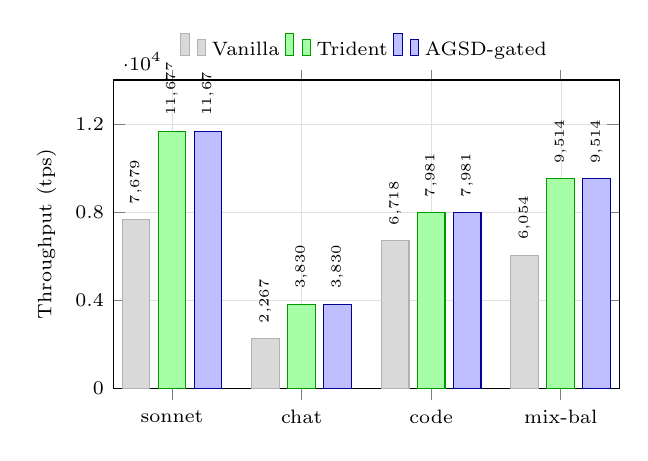
\begin{tikzpicture}
\begin{axis}[
    ybar=3pt,
    bar width=10pt,
    width=8cm, height=5.5cm,
    ylabel={Throughput (tps)},
    ylabel style={font=\scriptsize},
    symbolic x coords={sonnet, chat, code, mix-bal},
    xtick=data,
    xticklabel style={font=\scriptsize},
    yticklabel style={font=\scriptsize},
    ymin=0, ymax=14000,
    ytick={0,4000,8000,12000},
    legend style={at={(0.5,1.03)}, anchor=south, legend columns=3,
                  font=\scriptsize, draw=none},
    nodes near coords,
    nodes near coords style={font=\tiny, rotate=90, anchor=west, xshift=2pt},
    enlarge x limits=0.15,
    grid=major,
    grid style={line width=0.1pt, draw=gray!25},
]
\addplot[fill=gray!30, draw=gray!60] coordinates {
    (sonnet,7679) (chat,2267) (code,6718) (mix-bal,6054)};
\addplot[fill=green!35, draw=green!60!black] coordinates {
    (sonnet,11677) (chat,3830) (code,7981) (mix-bal,9514)};
\addplot[fill=blue!25, draw=blue!60!black] coordinates {
    (sonnet,11677) (chat,3830) (code,7981) (mix-bal,9514)};
\legend{Vanilla, Trident, AGSD-gated}
\end{axis}
\end{tikzpicture}%
}
\caption{Llama-3.3-70B + TP=8 + H100$\times$8 처리량 비교.
  Trident core가 모든 워크로드에서 vanilla 대비 $+18.8\%$--$+68.9\%$를 달성한다.
  Llama-70B는 전 워크로드에서 suffix가 최적이므로 AGSD $\equiv$ Trident.}
\label{fig:throughput-gain}
\end{figure}
